% ============================================  CONFIGS  ==============================================

\documentclass[a4paper, 11pt]{article}

% ============================================  USERSETTINGS  ==========================================

\newcommand{\myTitle}{Small \LaTeX{} Article Template\xspace}
\newcommand{\mySubtitle}{Subtitle\xspace}
\newcommand{\myDegree}{Degree\xspace}
\newcommand{\myName}{First Name Last Name\xspace}
\newcommand{\myProf}{Prof. Name\xspace}
\newcommand{\myOtherProf}{Prof. Name\xspace}
\newcommand{\mySupervisor}{Supervisor Name\xspace}
\newcommand{\myFaculty}{Faculty\xspace}
\newcommand{\myDepartment}{Department\xspace}
\newcommand{\myUni}{University\xspace}
\newcommand{\myLocation}{Location, Country\xspace}
\newcommand{\myTime}{\today\xspace}
\newcommand{\myVersion}{version 1.0\xspace}

% === USERSETTINGS FORMATTING: TITLE === 
\title{\vspace{-15mm}\fontsize{24pt}{10pt}\selectfont\textbf{\myTitle}} % Article title

\author{
\large
\textsc{\myName}\\[2mm]
\normalsize \myUni \\
\normalsize \myFaculty \\ 
\normalsize \href{mailto:test@test.com}{test@test.com} % change to your mail
\vspace{-5mm}
}
\date{}


% ============================================  PACKAGES  ==============================================

% === TEMPLATE RELATED: Remove in case of usage! ===
\usepackage{lipsum} % Package to generate dummy text throughout this template

% === %unsorted% ===
\usepackage{filecontents}


% === FONT & LANGUAGE ===
% \usepackage[ngerman]{babel} % set language
\usepackage[main=english,ngerman]{babel} % set multi-language document

\usepackage{microtype} % Slightly tweak font spacing for aesthetics
\usepackage[utf8]{inputenc}
\usepackage[T1]{fontenc} % needed if Umlauts are used
\usepackage[utf8]{inputenc}
\usepackage{lmodern}
\usepackage{xspace} % adds a space unless the macro is followed by certain punctuation characters

% === MARGINS ===
\usepackage[a4paper]{geometry}
\geometry{left=2.5cm,right=2.5cm,top=2.4cm,bottom=2cm}%Seitenränder
\usepackage[onehalfspacing]{setspace}%Zeilenabstand
\renewcommand{\\}{\vspace*{0.5\baselineskip} \newline}

% === MULTICOLUMN ===
\usepackage{multicol} 

% === CITATION ===
\usepackage[
  backend=biber,
  citestyle=ieee
]{biblatex}
\addbibresource{bibliography.bib} %Imports 

% === Abstract ===
\usepackage{abstract} % Allows abstract customization
\renewcommand{\abstractnamefont}{\normalfont\bfseries} % Set the "Abstract" text to bold
\renewcommand{\abstracttextfont}{\normalfont\small\itshape} % Set the abstract itself to small italic text

% === SECTIONS ===
\renewcommand\thesection{\Roman{section}} % sections with roman numerals
\renewcommand\thesubsection{\Roman{subsection}} % subsections with roman numerals
%\titleformat{\section}[block]{\large\scshape\centering}{\thesection.}{1em}{} % new style of section titles
%\titleformat{\subsection}[block]{\large}{\thesubsection.}{1em}{} % new style of section titles

% === HEADERS & FOOTERS
%\usepackage{fancyhdr} 
%\pagestyle{fancy} % set for all pages
%\fancyhead{} % Blank out the default header
%\fancyfoot{} % Blank out the default footer
%\fancyhead[C]{Running title $\bullet$ November 2012 $\bullet$ Vol. XXI, No. 1} % Custom header text
%\fancyfoot[RO,LE]{\thepage} % Custom footer text

% === FIGURES ===
\usepackage{graphicx}

% === TABLES ===
\usepackage{booktabs}  % Horizontal rules in tables
\usepackage{array} % extends tabular

% === ROTATION ===
\usepackage{rotating}

% === Algorithms ===
\usepackage{algorithm}
\usepackage{algorithmic}

% === Hyperlinks ===
\usepackage[hidelinks,breaklinks]{hyperref}

% === FIXES ===
\newcommand{\theHalgorithm}{\arabic{algorithm}} % hyperref and algorithmic misbehave sometimes
\usepackage{float} % Required for tables and figures in the multi-column environment - they need to be placed in specific locations with the [H] (e.g. \begin{table}[H])
\usepackage{paralist} % less space between bullet points

% ============================================  FINETUNING  =============================================

%\renewcommand*{\backref}[1]{}
%\renewcommand*{\backrefalt}[4]{{\footnotesize [%
%    \ifcase #1 Not cited.%
%    \or Cited on page~#2%
%    \else Cited on pages #2%
%    \fi%
%]}


% ============================================  DOCUMENT  =============================================

\begin{document}

% ===  TITLE  ===
\maketitle

% === ABSTRACT ===
\begin{abstract}
	\noindent \lipsum[1] % remove dummy text
\end{abstract}

\begin{multicols}{2} % start multicolumn layout

% ===  CONTENT  ===

% section
\section{Introduction}\label{sec:intro}
\lipsum*[2-3] % remove dummy text

% subsection
\subsection{Detail}

\begin{compactitem}
	\item Donec dolor arcu, rutrum id molestie in, viverra sed diam
	\item Curabitur feugiat
	\item turpis sed auctor facilisis
	\item arcu eros accumsan lorem, at posuere mi diam sit amet tortor
	\item Fusce fermentum, mi sit amet euismod rutrum
	\item sem lorem molestie diam, iaculis aliquet sapien tortor non nisi
	\item Pellentesque bibendum pretium aliquet
\end{compactitem}
\lipsum[4] % remove dummy text

% paragraph
\paragraph{Paragraph}
\lipsum[75]

\begin{description}
	\item[article\label{article}]{Article is \ldots}
	\item[book\label{book}]{the book class is \ldots}
	\item[report\label{report}]{class report does \ldots}
	\item[letter\label{letter}]{for german letters you should use something else}
\end{description}
	



% citation example
\section{Citation}\label{sec:cite}

This work~\cite{doe2006test} is great.

% table example
\section{Tables}\label{sec:tab}

\begin{table}[H]
	\caption{Example table}
	\centering
	\begin{tabular}{llr}
		\toprule
		\multicolumn{2}{c}{Name} \\
		\cmidrule(r){1-2}
		First name & Last Name & Grade \\
		\midrule
		John & Doe & $7.5$ \\
		Richard & Miles & $2$ \\
		\bottomrule
	\end{tabular}
\end{table}

\lipsum[5] % remove dummy text


% figures example
\section{Figures}\label{sec:fig}

\begin{figure}[H]
	\centering
	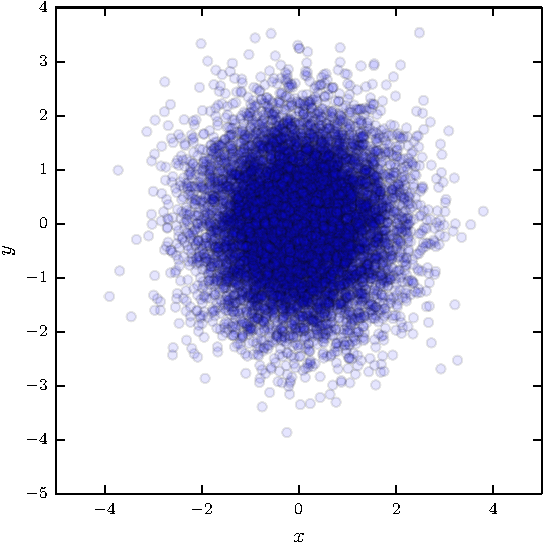
\includegraphics[width=0.9\columnwidth]{assets/figure_rasterized.pdf}
	\caption{Example of a rasterized plot}
\end{figure}

\lipsum[6] % remove dummy text

\section{Conclusion}\label{sec:conclusion}

\lipsum[7] % remove dummy text
\LaTeX{} Example by XYZ~\cite{doe2006test}.

% figures equations
\section{Equations}\label{sec:eq}
\begin{equation}
	\label{eq:emc}
	e = mc^2
\end{equation}


% ============================================  BIBLIOGRAPHY  ==============================================

\printbibliography

% ==========================================================================================================


\end{multicols}
\end{document}
